\section{Second-Order Tensor Field Visualization} % (fold)
\label{sec:tensor_fields}
%
Although tensors are a very general concept in mathematics, when we talk about
tensor fields in scientific visualization, we generally mean a map $\mT(\vx, t):
D \times T \mapsto \RRSet^{m \times m}$ from spatial domain $D \in \EESet^n$ and
temporal domain $T \in \RRSet$ to the space of second-order tensors which can be
represented by matrices from $\RRSet^{m \times m}$.
%
While a vector describes an effect acting on a point, a second-order tensor
describes an effect on a vector.
%
Often, this means that the tensor describes some sort of differential effect
that acts on the infinitesimal neighborhood of a point.
%
Second-order tensor fields occur in a variety of different scientific contexts.
%
Some examples are stress and strain tensors in mechanical engineering
applications, and diffusion tensors occurring in \ac{DTI}, a special \ac{MRI}
modality used to visualize fiber tracts, \eg, in the human brain.
%
In reality, these tensor fields vary in time.
%
However, in practice datasets with temporally varying tensor fields are
relatively rare, and visualization methods are mostly designed for instantaneous
tensor fields $\mT(\vx)$.
%

%
The most important tensor field visualization methods can be roughly classified
into five different categories:
%
direct, image-based, glyph-based, line-/surface-based and topology-based.
%

\subsection{Direct Methods} % (fold)
\label{sub:tensor_direct_methods}
%
Direct methods display some properties of the tensor directly.
%
Usually, one or more scalar quantities are derived from the vector field and
displayed using methods from scalar field visualization.
%
Notable examples for direct methods are \emph{color-mapping} and \emph{direct
volume rendering}.
%

%
\subsubsection{Color-Mapping} % (fold)
%
Just like scalar and vector fields, \ac{2D} or slices of \ac{3D} tensor fields
can be displayed by color-mapping some scalar properties of the tensor.
%
When investigating mechanical stress tensors, some norm of the tensor is often
displayed.
%
When viewing diffusion tensors from \ac{DTI} data, the \ac{3D} direction of the
major eigenvector is often encoded using a radial or spherical color
map~\cite{Pajevic1999}.
%
Such a visualization is not very intuitive and requires the viewer to be
familiar with the interpretation of the resulting images.
%
% subsubsection color_mapping (end)
%

\subsubsection{Direct Volume Rendering} % (fold)
%
For \ac{3D} data, the equivalent of color-mapping is direct volume rendering.
%
The additional degrees of freedom of a tensor compared to scalar or vector data
means that some information invariably gets lost when using normal direct volume
rendering techniques.
%
This means an intelligent mapping of the tensor to color, opacity and shading
needs to be performed to retain the most important aspects of the data.
%
For diffusion tensors, different possibilities for such mappings have been
explored by Kindlmann \etal{}~\cite{Kindlmann2000}.
%
They base their mappings on the different kinds of anisotropies indicated by the
ratio of the tensor's eigenvalues that can be found in diffusion tensor data
(namely linear anisotropy, planar anisotropy, and isotropy).
%
This produces visualizations that represent the important features in \ac{DTI}
data, but is not necessarily applicable to other application domains.
%
% subsubsection direct_volume_rendering (end)
% subsection direct_methods (end)

\subsection{Image-Based Methods} % (fold)
\label{sub:tensor_image_based}
%
Like the equivalent techniques for vector fields, image-based visualization of
second-order tensor fields works by generating space-filling images that are
derived from the underlying tensor data.
%
Techniques in this category have yet to be adopted into mainstream visualization
tools, so we will only discuss two notable examples: \emph{HyperLIC} by Zheng
and Pang~\cite{Zheng2003} and \emph{LIC with variable input textures} by Hotz
\etal{}~\cite{Hotz2004}.
%
Both techniques are modified versions of \ac{LIC} based on the eigenvectors of
the tensor fields.
%

\subsubsection{HyperLIC} % (fold)
%
HyperLIC was introduced by Zheng and Pang~\cite{Zheng2003} as a visualization
technique for diffusion tensor data.
%
In this data, a central characteristic is the diffusion anisotropy represented
by the ratio of the eigenvalues.
%
While \ac{LIC} accumulates the values of an input texture along streamlines of a
vector field, HyperLIC conceptually accumulates values in a strip- or tube-like
volume that follows the local eigenvector direction and whose cross section is
scaled according to the local eigenvalue ratio.
%
This produces \ac{LIC}-like results in areas with a strongly dominating
eigenvalue, and blurry areas with no sense of direction in isotropic areas where
all eigenvalues are similar.
%
As this technique is designed for diffusion tensors, which are positive
definite, it lacks a way of indicating eigenvalue sign and therefore is not well
suited for the visualization of indefinite tensors.
%
% subsection tensor_image_based (end)

\subsubsection{\ac{LIC} with Variable Input Textures} % (fold)
\label{ssub:lic_with_variable_input_textures}
%
A technique which is better suited for symmetric indefinite tensors, which can
have negative eigenvalues, was presented by Hotz \etal{}~\cite{Hotz2004}.
%
As opposed to HyperLIC, which accumulates the values of the input texture in a
volume instead of along a curve, this method uses a standard \ac{LIC} on the
``eigenvector fields'' of the tensor field.
%
The remaining information in the tensor is visualized by carefully varying the
spot size, spot density and color of the input noise texture as well as the
convolution length based on the local eigenvalues.
%
Images from major and minor eigenvector are overlaid to visualize both at the
same time.
%
\Cref{fig:lic_var_tex} shows an example of this technique applied to a slice
of the stress tensor field from a two point load dataset with a pushing and
pulling force.
%
\begin{figure}[t]
    % \centering
    \begin{captionbeside}{LIC with variable input textures. Image source: Hotz
    \etal{}~\cite{Hotz2004}.\label{fig:lic_var_tex}}
        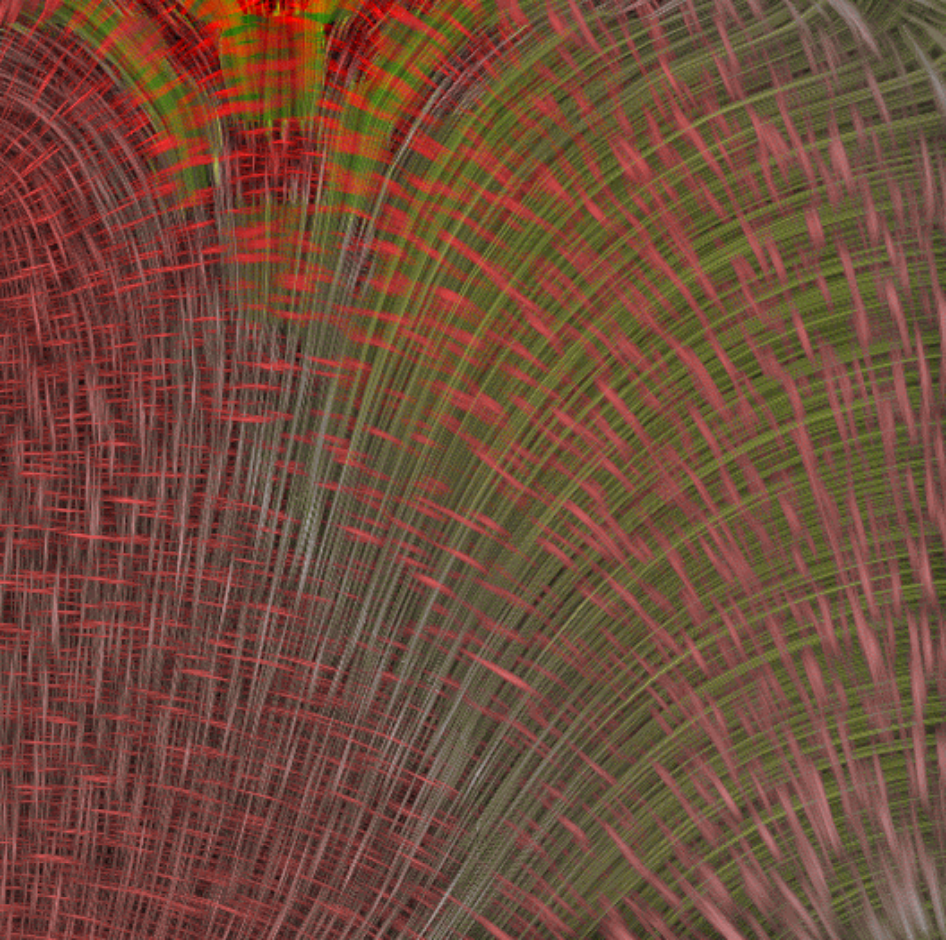
\includegraphics[width=0.6\textwidth]{figures/tensor_lic_variable_texture.png}
    \end{captionbeside}
    % \caption{LIC with variable input textures showing a stress tensor field of a
    % two point load dataset with a pushing and pulling force. Red shows negative
    % eigenvectors (compressive stress), green shows positive eigenvectors
    % (tensile stress). Density, spot size, color intensity and convolution length
    % are varied according to the local eigenvalues. Image source: Hotz
    % \etal{}~\cite{Hotz2004}.}
\end{figure}
%
% subsubsection lic_with_variable_input_textures (end)

\subsection{Glyph-Based Methods} % (fold)
\label{sub:tensor_glyph_based}
%
Glyph-based methods for tensor field visualization place small geometric objects
in space to represent certain characteristics of the local tensor.
%
They have the advantage of being able to display all features of a tensor at
once, but their visual complexity can make them hard to read.
%
Glyph-based methods generally differ by the restrictions they place on the
tensor.
%
There are various glyph designs for \emph{symmetric positive definite},
\emph{symmetric (indefinite)}, and \emph{general tensors} in both \ac{2D} and
\ac{3D}.
%
Some research has also focused on how to place and distribute glyphs to better
emphasize global structures in the data, as opposed to the simple regular
grid-based approach~\cite{Kindlmann2006,Feng2008}.
%

\subsubsection{Symmetric Positive Definite Tensors} % (fold)
%
Symmetric positive definite tensors are tensors that always have positive
real eigenvalues, and whose eigenvectors are orthogonal.
%
The domain most explored in scientific visualization for these tensors is
\ac{DTI} data, where they represent the diffusion of Hydrogen atoms in organic
tissue (specifically in neural fibers of the brain).
%
The simplest glyphs for visualizing such tensors are ellipses~\cite{Basser1996},
cylinders~\cite{Wiegell2000} or boxes~\cite{Schroeder2006}.
%
These glyphs are formed by placing some prototypical base shape (a unit sphere
or cube) centered at the origin and then transforming it according to the
tensor.
%
The resulting glyph is then placed at the sampling position the tensor
originated from.
%
Most often, the glyphs are also scaled to achieve a size fitting with the
glyph density.
%
Such simple glyphs accurately represent how the tensor transforms input vectors
to output vectors.
%
The disadvantage is that they have various visual ambiguities that make their
interpretability less than ideal~\cite{Kindlmann2004}.
%

%
Kindlmann~\cite{Kindlmann2004} solved this problem by carefully designing
glyphs based on superquadrics.
%
These superquadrics change their base shape depending on the relationship of
the three eigenvalues of the tensor.
%
In this way, ambiguities intrinsic to the usage of constant base shapes are
eliminated.
%

\subsubsection{Symmetric Tensors} % (fold)
%
General symmetric tensors always have real orthogonal eigenvectors, but their
eigenvalues can be negative.
%
This poses a challenge for glyph design.
%
Simply transforming a symmetric base shape with the tensor will produce the same
image for eigenvalues with equal magnitude but opposite sign.
%
Different glyphs for symmetric tensors in different application domains have
been proposed in the literature~\cite{Pajevic1999,Hashash2003,Jeremic2002}.
%
Often, color is used to indicate the sign of the eigenvalue.
%
Alternatively, the glyph base shape is modified to represent the difference
between positive and negative eigenvalues.
%
Schultz and Kindlmann~\cite{Schultz2010a} built on top of all of this work to
develop a set of superquadric-based tensor glyphs that clearly indicates
eigenvalue sign by a combination of color and concave shape (see
\cref{fig:tensor_glyphs}).
%
% \begin{figure}[t]
%     \begin{tikzpicture}
%         \node (pos) {
%             \includegraphics[width=0.3\textwidth]{figures/diffusion_tensor_glyphs.png}
%         };
%         \node[anchor=west] (symm) at (pos.east) {
%             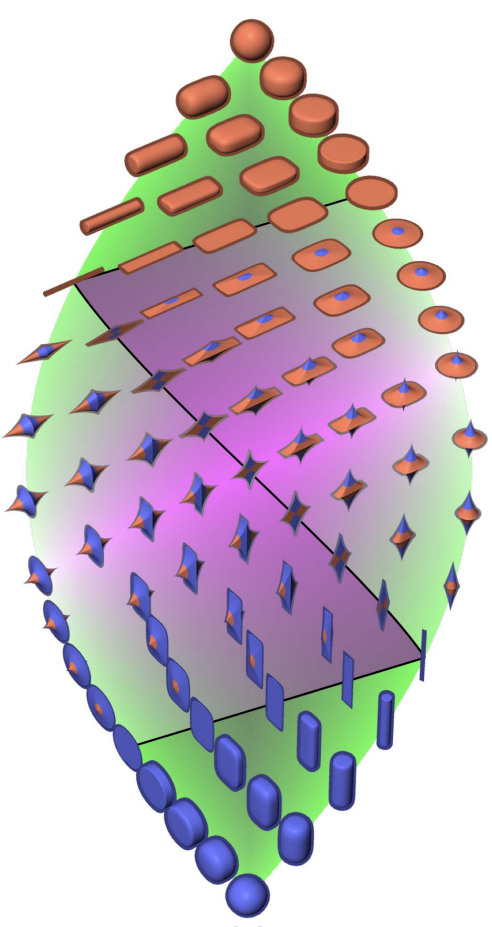
\includegraphics[width=0.3\textwidth]{figures/symmetric_tensor_glyphs.png}
%         };
%         \node[anchor=west] (general) at (symm.east) {
%             \includegraphics[width=0.3\textwidth]{figures/general_tensor_glyphs.png}
%         };
%     \end{tikzpicture}
%     \caption{Superquadric tensor glyphs for symmetric positive definite (left),
%     symmetric indefinite (middle), and general (right) tensors.}
%     \label{fig:tensor_glyphs}
% \end{figure}
%
% \begin{figure}[t]
%     \centering
%     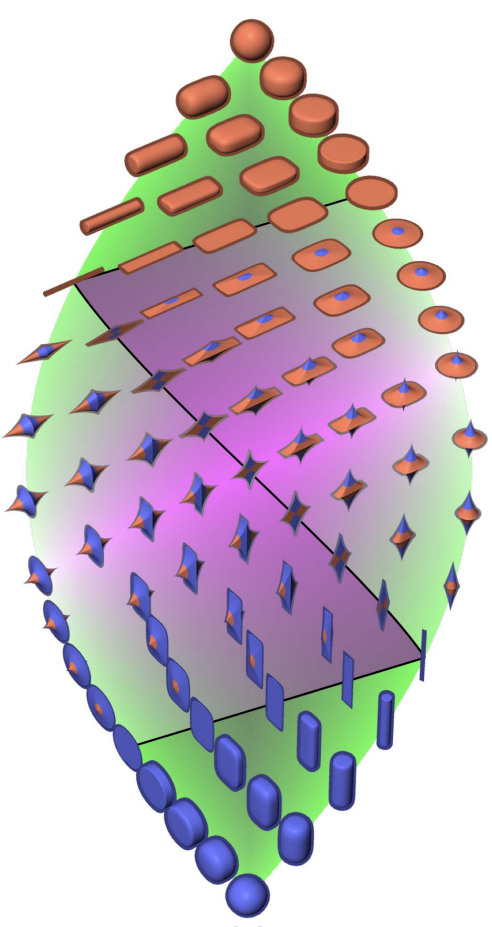
\includegraphics[width=0.5\textwidth]{figures/symmetric_tensor_glyphs.png}
%     \caption{Superquadric glyphs for symmetric tensors. Image source: Schultz
%     \etal{}~\cite{Schultz2010a}.}
%     \label{fig:tensor_glyphs}
% \end{figure}
%
\begin{figure}
    \begin{captionbeside}
        {Superquadric glyphs for symmetric tensors. Includes glyphs for positive
         definite tensors as a subset (top triangle). Image source: Schultz
         \etal{}~\cite{Schultz2010a}.\label{fig:tensor_glyphs}}
        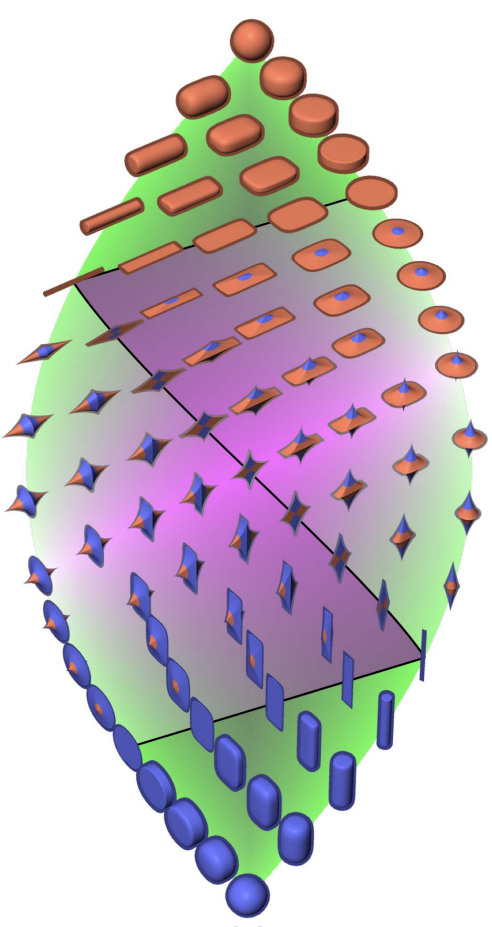
\includegraphics[width=0.4\textwidth]{figures/symmetric_tensor_glyphs.png}
    \end{captionbeside}
\end{figure}

\subsubsection{General Tensors} % (fold)
%
Apart from different eigenvalue signs, the eigenvectors of general (asymmetric)
second-order tensors need not be orthogonal, and they can be complex.
%
Gerrits \etal{}~\cite{Gerrits2017} built on top of the work of Kindlmann, Schultz
\etal{} to design a set of glyphs for general tensors in \ac{2D} and \ac{3D} that
can represent non-orthogonal eigenvectors and additionally incorporates
information about complex eigenvalues via color.
%

\subsection{Line-/Surface-Based Methods} % (fold)
\label{sub:tensor_line_surface_based}
%
Line- and surface-based methods for the visualization of second-order tensor
fields are very similar to integral lines and surfaces for vector fields.
%
They work by considering the eigenvectors of the tensor field as the equivalent
of a vector field and basing the visualization on the resulting field lines.
%
Of course these methods can only visualize real eigenvectors and are therefore
generally applied to symmetric tensor fields only.
%
Because of the differences between real vector fields and eigenvector fields,
modified integration methods are necessary to form these field lines.
%
The most important methods based on this principle are \emph{tensor field
lines}, \emph{hyperstreamlines}, \emph{tensorlines} and
\emph{hyperstreamsurfaces}.
%

\subsubsection{Tensor Field Lines} % (fold)
%
Tensor field lines are lines that are everywhere tangent to an eigenvector of
the tensor field.
%
They are the basis for all the methods in this category.
%
Tensor field lines have been known as \emph{stress trajectories} (see
\cref{fig:stress_trajectories}) in the context of solid mechanics since the
1800s.
%
Early stress visualizations using this technique were drawn by hand based on
photoelastic measurement techniques~\cite{Focht1962,Timoshenko1983}.
%
In a computer, these lines are obtained by integrating a vector field generated
from the eigenvector field by choosing an orientation and magnitude at each
location \cite{Dickinson1989,Tricoche2006}.
%
Since this choice is not always unique in the vicinity of degenerate points
where two or more eigenvalues are equal, special care has to be taken to avoid
a sudden flip of direction.
%
The resulting lines show the continuous change of direction of eigenvectors in
the tensor field, but they are not well suited to judge the magnitude of the
eigenvalues.
%
\begin{figure}[t]
    \centering
    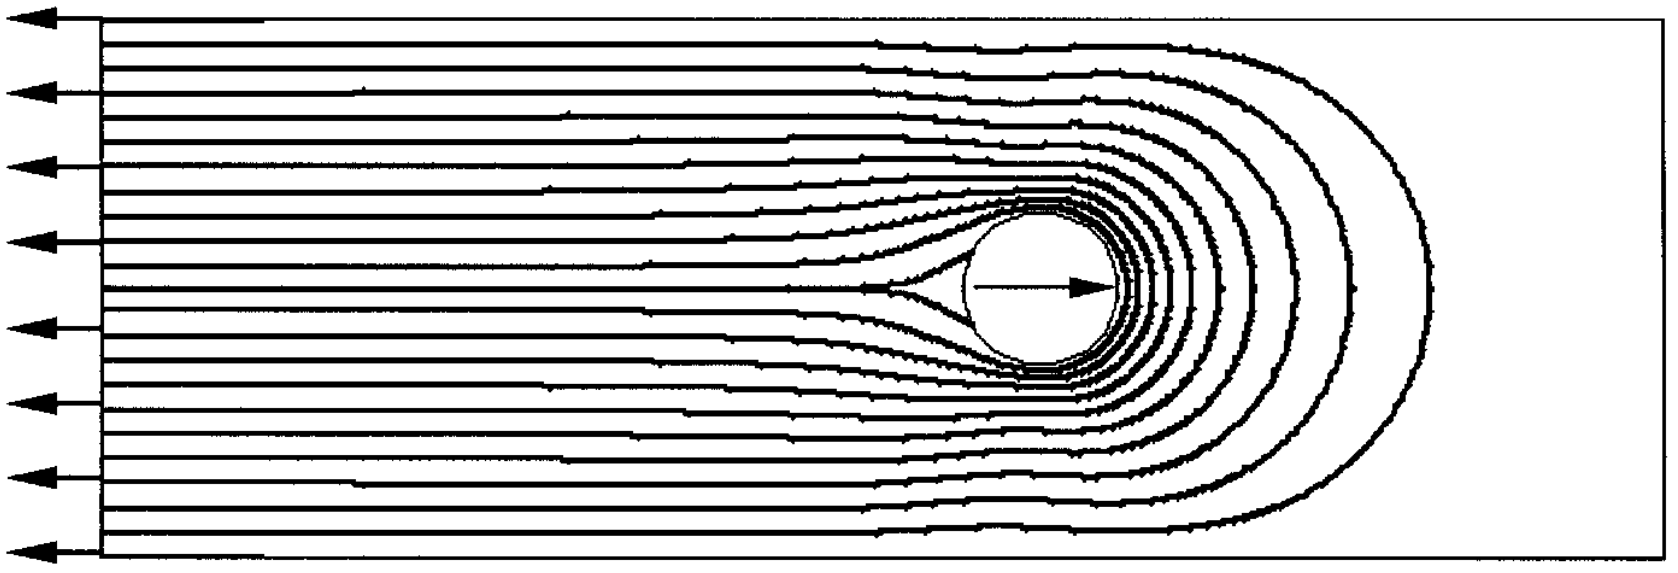
\includegraphics[width=0.8\textwidth]{figures/stress_trajectories.png}
    \caption{Major principal stress trajectories in a plate with a loaded hole.
             Image source: Kelly and Tosh~\cite{Kelly2000}.}
    \label{fig:stress_trajectories}
\end{figure}
%

\subsubsection{Hyperstreamlines} % (fold)
%
To enhance the information content of tensor field line visualizations,
Delmarcelle and Hesselink introduced hyperstreamlines~\cite{Delmarcelle1993}.
%
These hyperstreamlines follow the field lines of one of the eigenvectors of the
tensor field, while their cross-section is a cross shape or ellipse aligned with
the other two eigenvectors and scaled by the corresponding eigenvalues.
%
The eigenvalue corresponding to the eigenvector parallel to the hyperstreamline
is color-coded on the surface.
%
In this way, the full information of the tensors along the hyperstreamlines is
visualized.
%
It is important to note here that the term hyperstreamline is sometimes used
in the literature to mean what we introduced as tensor field lines.
%
In this work, we use it exclusively for lines with a variable cross-section.
%

\subsubsection{Tensorlines} % (fold)
%
In the analysis of diffusion tensor fields obtained from \ac{DTI} scans of the
human brain, tensor field lines are tracked to obtain the paths of neural
fibers.
%
Because this data suffers from noise and partial voluming effects due to limited
resolution, near-isotropic areas can occur where fibers with different
directions cross.
%
In these areas, the eigenvector direction is not clearly defined and often
dominated by noise.
%
Just following the vector field obtained from a single eigenvector will result
in random paths that do not represent the paths of actual brain fibers.
%
To counteract this problem, Weinstein \etal{}~\cite{Weinstein1999} introduced
tensorlines.
%
The core of the algorithm is a modified streamline integration that not only
takes into account the direction of the major eigenvector but is also guided
by the direction of the previous step in near-isotropic regions.
%

\subsubsection{Hyperstreamsurfaces} % (fold)
%
The concept of hyperstreamlines was extended to hyperstreamsurfaces by Jeremi\'c
\etal{}~\cite{Jeremic2002}.
%
They are formed analogous to streamsurfaces by using a curve instead of a point
as a seed structure for integration.
%
In this case, the other eigenvectors and eigenvalues can not be sensibly
displayed by varying a cross section like with hyperstreamlines.
%
Instead, only the eigenvalue of the integrated eigenvector is color-coded on the
surface.
%

\subsection{Topological Methods} % (fold)
\label{sub:tensor_topological}
%
Similar to scalar- and vector fields, topological structures in tensor fields
are defined by some mathematical degeneracy.
%
In contrast to the topology of vector fields, it is not the magnitude of the
tensor that is important, but the relationship between the eigenvalues and
eigenvectors.
%
For symmetric tensor fields, the topology is formed by \emph{degenerate points
and lines} and their \emph{separatrices}, as well as \emph{neutral and traceless
tensors}.
%
For \emph{general (asymmetric) tensor fields}, the topology is formed by
degenerate structures and circular points.
%

\subsubsection{Degenerate Points and Lines} % (fold)
%
The core of topological analysis of symmetric tensor fields are degenerate
structures.
%
These are structures where two eigenvalues are equal, and the eigenvector
directions are not uniquely defined.
%
They are the locations where tensor field lines intersect.
%
In \ac{2D} tensor fields, such structures can be classified into trisector and
wedge points, depending on the behavior of the tensor field lines in their
vicinity.
%
In \ac{3D}, degenerate features form lines.
%
Zheng \etal{}~\cite{Zheng2005b} showed that the type of degenerate point can
switch at isolated points along these lines.
%
These are the points where the degenerate line is parallel to the plane spanned
by the valid eigenvectors corresponding to the dual eigenvalue.
%
Degenerate lines in symmetric tensor fields were first studied by Delmarcelle,
Hesselink \etal{}~\cite{Delmarcelle1994,Hesselink1997}.
%
Numerical algorithms for their robust extraction were developed by Zheng
\etal{}~\cite{Zheng2004,Zheng2005} and later adapted for noisy \ac{DTI} data by
Tricoche \etal{}~\cite{Tricoche2008}.
%
\Cref{fig:tensor_topology} shows the topology of a common test case in
structural mechanics where two point loads are applied to the surface of a solid
block.
%
\begin{figure}[t]
    \begin{captionbeside}
        {Topology of the stress tensor in a double point load dataset. Image
         source: Zheng and Pang~\cite{Zheng2004}.\label{fig:tensor_topology}}[o]
        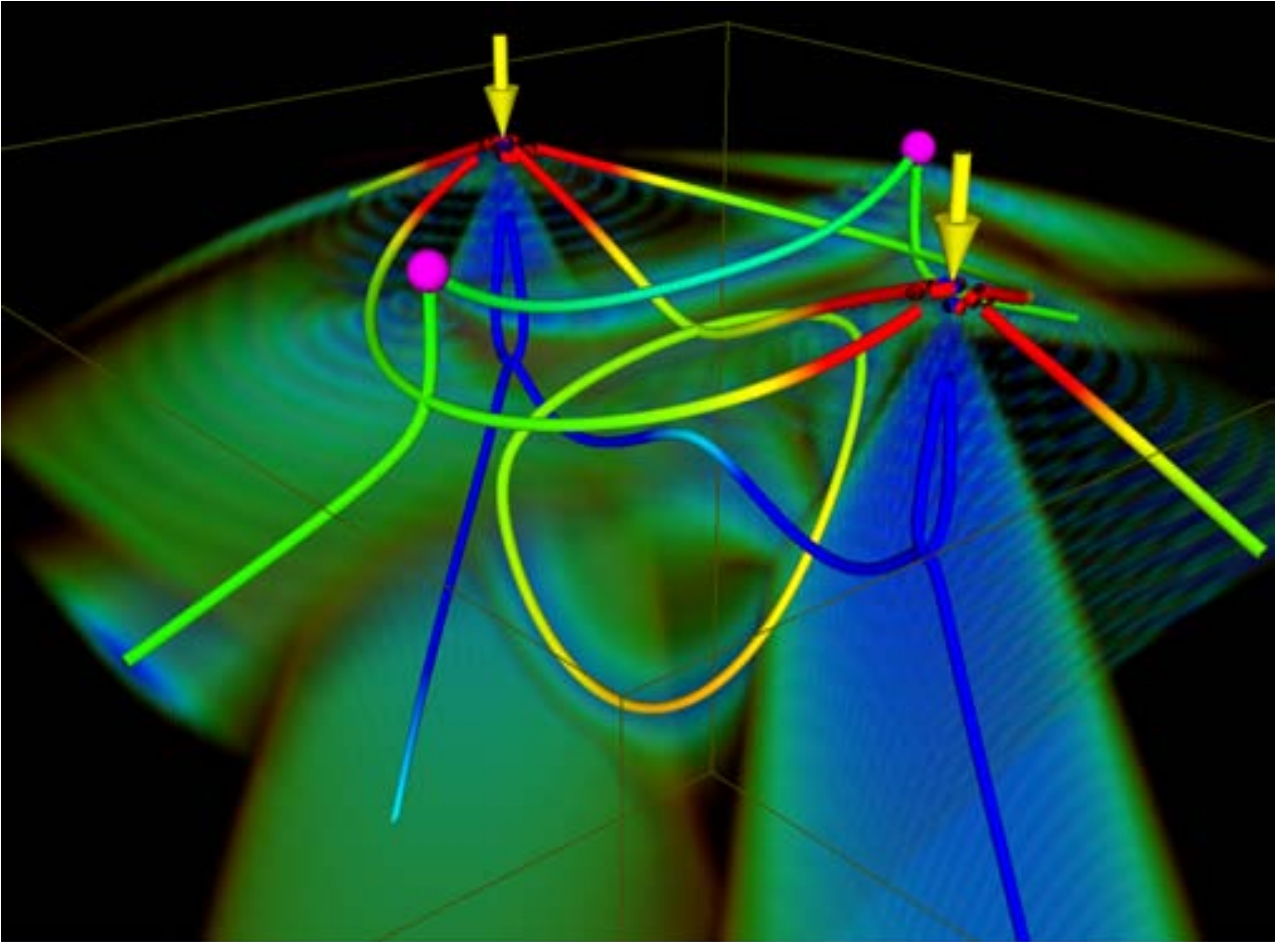
\includegraphics[width=0.6\textwidth]{figures/tensor_topology.png}
    \end{captionbeside}
\end{figure}
%

\subsubsection{Separatrices} % (fold)
%
The tensor field lines that pass through a degenerate point form separatrices
that separate the neighborhood of the point into sectors~\cite{Delmarcelle1994}.
%
These structures are akin to the separatrices of vector fields that separate
the area around a saddle point.
%
In \ac{2D}, these separatrices are lines, in \ac{3D}, they form surfaces.
%
An algorithm for extracting such surfaces from \ac{3D} tensor fields was
proposed by Zheng \etal{}~\cite{Zheng2005b}
%

\subsubsection{Neutral and Traceless Tensors} % (fold)
%
A different kind of topological feature are neutral and traceless tensors,
which were first investigated bu Palacios \etal{}~\cite{Palacios2016}.
%
A neutral tensor is a tensor where the middle eigenvalue is the average of the
major and minor eigenvalue.
%
Neutral tensors in \ac{3D} tensor fields form surfaces.
%
These surfaces mark the transition between areas of linear tensors (one
dominating eigenvalue) and planar tensors (two dominating eigenvalues).
%
In stress tensors, these can be interpreted as the transition between
predominantly tensile stress and predominantly compressive stress.
%
In diffusion tensors from \ac{DTI}, they indicate the separation between
regions with clear fiber direction and regions where fiber tracts cross.
%

%
Traceless tensors are tensors whose sum of eigenvalues is zero.
%
Traceless tensors also form surfaces in \ac{3D} tensor fields.
%
They mark the transition between areas of positive and negative trace.
%
In stress and strain tensors, these are equivalent to regions of expansion and
compression.
%
Recently, Roy \etal{}~\cite{Roy2019} proposed a more robust extraction method for
these surfaces as well as degenerate lines.
%

\subsubsection{Topology of General (Asymmetric) Tensor Fields} % (fold)
%
The topology of general tensor fields has been studied to a lesser extent.
%
Zheng and Pang~\cite{Zheng2005a} first introduced \emph{circular points} as the
main topological structure in \ac{2D} general tensor fields.
%
These are points where the tensor is a perfect rotation matrix.
%
Analogous to degenerate points in symmetric tensor fields, these are also points
where all vectors are valid eigenvectors.
%
Degenerate structures where two eigenvalues are equal also exist in general
tensor fields, but here they mark the transition between regions of real and
complex eigenvectors.
%
This means that they form lines instead of points in \ac{2D}, and their meaning
is very different.
%
Zhang \etal{}~\cite{Zhang2009} later extended the study of \ac{2D} general tensor
fields by defining eigenvector and eigenvalue manifolds to classify general
tensors and distinguish different types of circular points.
%
% subsection topological_methods (end)
%
% section tensor_fields (end)